\documentclass[a4paper,11pt]{report}

% HER BEGYNDER PRÆAMBLEN

% Skrivemaskinfont

\usepackage{courier}

% Farver

\usepackage{color}

\usepackage{listings}

\newcommand{\injava}[1]{\lstinline[language=Java]{#1}}

\lstnewenvironment{java} {\lstset{language=Java}} {}

% En pakke til lokalisering, herunder orddeling på andre sprog end
% amerikansk engelsk

\usepackage[danish]{babel}

% En nyttig matematik-pakke

\usepackage{amsmath}

% En anden nyttig pakke -- til opsætning af matematiske sætninger,
% definitioner mm.

\usepackage{amsthm}

% Symboler

\usepackage{amssymb}

% Ved brug af billedfiler

\usepackage{graphicx}

% Til hyperlinks

\usepackage{hyperref}

% Til ombrydning af lange URL'er

\usepackage{breakurl}
\usepackage{xspace}

% Til TikZ

\usepackage{tikz}

% Til automater i TikZ

\usetikzlibrary{arrows,shapes, calc}
\usetikzlibrary{automata}

% FILEN MED KOMMANDOER

%%% Local Variables:
%%% mode: LaTeX
%%% TeX-master: "report"
%%% End:

% Baseret på https://gist.github.com/mpdehnel/cc43e89a09c18ef6a602

\definecolor{mygreen}{rgb}{0,0.6,0}
\definecolor{mygray}{rgb}{0.5,0.5,0.5}
\definecolor{mymauve}{rgb}{0.58,0,0.82}
\definecolor{verylightgray}{gray}{0.92}

\lstset{ %
  backgroundcolor=\color{verylightgray},     % Baggrundsfarve; kræver pakken
                                                               % color - dvs. \usepackage{color} eller \usepackage{xcolor}
  basicstyle=\footnotesize\ttfamily,   % Skrivemaskine-font
  breakatwhitespace=false,                 % Intet linjeskift ved whitespace
  breaklines=true,                                % Automatisk linjeskift
  captionpos=b,                                    % Caption sat nederst i bunden
  commentstyle=\color{mygreen},     % Kommentarer med grøn
  escapeinside={\%*}{*)},                     % LaTeX-escape til hvis
                                                               % man får brug for LaTeX-kommandoer i koden
  extendedchars=true,                         % Tillader ikke-ASCII-tegn. Virker IKKE med UTF-8.
  frame=single,                                      % Ramme om koden.
  keywordstyle=\color{blue},               % Reserverede ord med blåt
  numbers=left,                                     % Linjenummerering mod venstre
  numbersep=5pt,                                % Afstand mellem linjenumre og kode
  numberstyle=\tiny\color{mygray},   % LInjenumre med grå
  rulecolor=\color{black},                     
  showspaces=false,                             
  showstringspaces=false,           
  showtabs=false,
  stepnumber=1,                    % Hver linje får et nummer
  stringstyle=\color{mymauve},     
  tabsize=2,
  title=\lstname                   
}

%%% Local Variables:
%%% mode: latex
%%% TeX-master: "report"
%%% End:

\newcommand{\bibtex}{\mbox{\textsc{BiB}\TeX}\xspace}
\newcommand{\latex}{\LaTeX\xspace}

\newcommand{\fig}[1]{Figur \ref{#1}}
\newcommand{\afs}[1]{Afsnit \ref{#1}}

\newcommand{\svar}{\paragraph{Svar:}}

\theoremstyle{definition}
\newtheorem{ovelse}{Øvelse}[chapter]

%%% Local Variables:
%%% mode: latex
%%% TeX-master: "report"
%%% End:


\title{Et kort dokument om \LaTeX}
\author{Hans}

\date{Februar 2026}






% HER BEGYNDER DOKUMENTDELEN

\begin{document}

\maketitle

\tableofcontents

\chapter*{Forord}

I min tid som censor på de danske datalogiuddannelser har jeg opdaget
noget påfaldende: Datalogiuddannelsen på RUC er det eneste sted i den
danske universitetsverden, hvor de fleste studerende bruger Microsoft
Word i stor stil. De fleste kender ikke til \latex og ved ikke, hvad
dette system tilbyder. Resultatet er kluntet opsatte projektrapporter
og underlige, pølsede ad hoc-arbejdsgange, der slet ikke understøtter
gruppearbejde godt.

Denne tekst er et forsøg på at skabe en forandring til noget mere
passende. Teksten på en og samme tid 

\begin{itemize}
\item et eksempel på hvordan man kan bruge \latex til at skrive
  dokumenter med, når man studerer datalogi, og 
  
\item en guide til hvordan man kommer i gang med at bruge \LaTeX.
\end{itemize}

\chapter{Hvad er det her?}

I afsnit \ref{afs:hvad} forklarer vi forskellen på  \TeX, \latex  og
Overleaf. Og i afsnit \ref{afs:hvorfor} forklarer vi, hvorfor man bør
bruge disse systemer, når man laver projektarbejde på datalogi.
Endelig, i afsnit \ref{afs:komigang}, forklarer vi om filformater og
hvordan man kommer i gang med at skrive dokumenter i \LaTeX.

\section{ \TeX, \latex  og Overleaf} \label{afs:hvad}

\begin{description}
\item[\TeX] er et dokumentbehandlingssystem, der skyldes den
  amerikanske datalog og matematiker Donald Knuth. Han brugte \TeX\ i
  sin klassiker, flerbindsværket \emph{The Art of Computer
    Programming} \cite{knuth1997computer} og dokumenterede \TeX\ i en
  anden bog \cite{Knuth:1996}. Knuth fik ACM Turing Award, datalogiens
  svar på Nobelprisen, for sit arbejde med algoritmeteori,
  programmeringssprog og meget andet, så han er ikke helt dum.
\item[\LaTeX] er et dokumentbehandlingssystem, der skyldes den
  amerikanske datalog og matematiker Leslie Lamport. Lamport
  implementerede \latex  som en samling definitioner af kommandoer og
  environments, skrevet i \TeX. Han dokumenterede systemet i
  \cite{lamport86latex}, der samtidig er en god indføring\footnote{Og
    spørger man mig, er den stadig den bedste af slagsen.}. Knuth fik
  ACM Turing Award, datalogiens svar på Nobelprisen, for sit arbejde
  med teorier for specifikation og verifikation af distribuerede
  systemer, så han er heller ikke helt dum. Nogle mennesker er glade
  for \TeX, men de fleste bruger \LaTeX.

  \TeX\ og \latex  kan installeres på din egen computer, og du kan
  arbejde helt offline med systemet og bruge din yndlings-teksteditor
  som f.eks. Visual Studio Code eller Emacs sammen med det, præcis
  ligesom man kan med programmeringssprog. {\TeX}Live-distributionen
  er et godt valg for mange, hvis man vælger denne løsning.
  
\item[Overleaf] er en online-løsning, som blev til i 2011 og skyldes
  matematikerne John Hammersley og John Lees-Miller. Overleaf er en
  løsning, der rummer en flerbruger-editor og ikke kræver, at man selv
  installerer \TeX/\LaTeX. Mange studerende er glade for Overleaf af
  disse grunde og kan være et godt sted at starte.
\end{description}

\section{Hvad er det, \latex  er godt til?}\label{afs:hvorfor}

Mange, der ikke har brugt \latex  og lever i Word-land, tror, at
\latex  bare er en slags "system til pænt layout med bøvlet brugergrænseflade''.
Men sandheden er en ganske anden. 

\begin{description}
\item[Kollaborativ skrivning] En gruppe af studerende, der lever i Word-land,
  skaber ofte en projektrapport, der er en kæmpestor Word-pølse, som de deler i
  et Dropbox-katalog eller på anden vis.

  Men \latex  understøtter helt direkte modulær skrivning. Man kan
  dele et stort dokument op i mange små del-filer, som bliver samlet
  af en main-fil. Dette dokument er et eksempel på dette. \latex gør
  det muligt at gøre det, man \emph{egentlig gerne vil} i
  gruppearbejde. Hvis man i forvejen beskæftiger sig med
  programmering, ligner dette noget, man kender i forvejen.
  
\item[Automatisk styr på referencer] Noget af det, studerende i
  Word-land bruger\footnote{eller spilder} en masse tid på, er at
  opdatere krydsreferencer og litteraturhenvisninger i Word-pølsen
  manuelt. Nogle studerende, der er begyndere udi \latex, tror at de
  skal være i besiddelse af en stor \latex-pølse, som de er nødt til
  at opdatere manuelt. Men \latex og \TeX\ er ud over mulighederne for
  modularitet designet til at håndtere alt dette automatisk, så alle
  ændringer kan håndteres automatisk af systemet. Man skal bruge tiden
  på at tænke over sit projekt, ikke på at skulle håndtere at Figur 17 skal hedde
  Figur 17 overalt i Word-pølsen.

\item[Simple tekstfiler] \LaTeX-filer er \textsl{tekstfiler}, og de er meget
  små. Selv små Word-pølser fylder temmelig meget. Min PhD-afhandling
  fylder, alt inklusive, er 124 sider lang og fylder omkring 1
  megabyte. Enhver \LaTeX- eller \TeX-fil kan åbnes i en vilkårlig
  teksteditor som Emacs, Vim, Notepad eller Visual Studio Code.

  Tekstfiler gør det muligt at bruge versionskontrol som Git til
  kollaborativ skrivning på præcis samme måde som man kan bruge Git
  til versionskontrol af programkode.

\item[Bibliografi-databaser] \latex  er udviklet sammen med \bibtex, Alle danske universiteter har
  universitetsbiblioteker, der tillader at man kan hente
  bibliografi-oplysninger i \bibtex-format. Også de store
  bibliografiservere som ACM Digital Library \cite{acmdl} og DBLP
  \cite{dblp} tillader dette. På den måde kan man hente filer med
  udtømmende oplysninger om sine
  kilder i stedet for selv at skulle bøvle med at stykke oplysningerne sammen.

\item[Egne kommandoer] \latex  er nem at udvide; det er muligt at lave
  nye kommandoer og environments, så man kan lave nye genveje til de
  samlinger af kommandoer, man ofte bruger. Hvis man i forvejen
  beskæftiger sig med programmering, ligner også dette noget, man
  kender i forvejen.
  
\item[Pakker] Fordi \TeX\ og \latex er nemme at udvide, findes der en
  hel masse udvidelser som gør det nemt at skrive

  \begin{itemize}
  \item programkode (\texttt{listings} og \texttt{minted}), som vi
    vender tilbage til i kapitel \ref{kap:kode}.
  \item pseudokode (\texttt{algorithm})
  \item indlejring og skalering af billedfiler (\texttt{graphicx}, som
    vi vender tilbage til senere)
  \item vektorgrafik (\texttt{tikz}, som reelt er et lille sprog i selv!)    
  \end{itemize}

\item[At skrive matematik] Alle hoved-personerne bag \TeX, \latex  og
  Overleaf er matematikere og har stor ekspertise inden for matematisk
  typografi. Skriver man matematik eller inden for andre fagområder,
  hvor man bruger matematik i stort omfang, er der ikke noget seriøst
  alternativ. Store sammenslutninger for fagmatematikere
  som f.eks. American Mathematical Society er med til at udvikle nye
  pakker til \LaTeX, og forlag, der udgiver faglitteratur inden for
  matematik og naturvidenskab (herunder datalogi), kræver som
  hovedregel, at forfattere bruger \LaTeX.
\end{description}

\section{Kom i gang med \LaTeX} \label{afs:komigang}

Alle er meget velkomne til at bruge denne tekst som udgangspunkt --
det er derfor, den er der.

\subsection{Strukturen af et \LaTeX-dokument}

En hovedfil består af to 
\begin{itemize}
\item En \emph{præambel} med pakke-importoplysninger, definitioner af
  nye kommandoer og environments mm.
\item En dokument-del, der er omkranset af
  \verb2\begin{document}...\end{document}2. I denne del findes selve
  teksten. 
\end{itemize}

I begge disse dele kan der være \verb2input2-kommandoer, der indlæser
underfiler. 

\subsection{Arbejdsgangen}

Oprindelig gjorde implementationer af \TeX\ og \latex det, at de
producerede en fil i dvi-format, som så skulle oversættes til en
Postscript-fil eller en PDF-fil.

Nyere implementationer som \texttt{pdflatex} springer dette led over
og producerer en PDF-fil direkte fra tex-filen.

\paragraph{Hvis man bruger kommandolinjen}

Hvis hovedfilen hedder \verb2rapport.tex2, kompilerer man den ved at
skrive

\begin{verbatim}
pdflatex rapport
\end{verbatim}

Denne kommando producerer en samling nye filer med forskellige
informationer og et (forsøg på) et renderet output. Se
\afs{subs:filer}.

\paragraph{Hvis man bruger Overleaf}

Hvis man bruger Overleaf, bliver dokumentet altid kompileret tre
gange, så citationer og krydsreferencer er blevet samlet rigtigt op. 

\subsection{Filformater} \label{subs:filer}.

\begin{description}
\item[tex] Filer med dette suffiks indeholder tekst, der bruger
  \LaTeX-kommandoer.
\item[aux] Filer med dette suffiks indeholder opsamlede data om referencer til
  figurer, formler, litteratur mm. Disse filer er arbejdsgangens
  "hukommelse'' og bruges til kompilering.
\item[blg] Hvis man bruger \bibtex, er dette en hjælpefil.
\item[bbl] Hvis man bruger \bibtex, er dette den bibliografi, der er
  blevet dannet.
\end{description}

En af filerne er en \verb2aux2-fil, der samler krydsreferencer og
kildehenvisninger. Den bliver genereret hver gang man kompilerer. Så
hvis man kompilerer for første gang eller ændrer på henvisninger, kan
man komme ud for at skulle kompilere én gang til og eventuelt for også
at skulle bruge \textsc{Bib}\TeX til at samle kildehenvisninger op.

\section{Det der med appendiks}

I en projektrapport eller en artikel har man tit brug for at placere
nogle dele af teksten i et appendiks. Sæt kommandoen \verb2\appendix2
der, hvor appendikserne skal begynde. Derefter bliver alle kapitlet
nummereret med bogstaver.

%%% Local Variables:
%%% mode: latex
%%% TeX-master: "report"
%%% End:

\chapter{Om at skrive matematik}

I \LaTeX\ skelner man mellem LR-mode (til brødtekst) og mathmode.

\section{Inline vs. display-matematik}

Matematik skrevet midt i en sætning kalder man \emph{inline}-matematik og
skrives mellem dollartegn: \texttt{\$ ... \$}. For eksempel giver
\texttt{\$f(n) = O(n \^{} 2)\$} resultatet $f(n) = O(n^2)$.
 
Hvis matematikken skal stå for sig selv på egen linje, bruges
\emph{display}-matematik med \texttt{\textbackslash[ ... \textbackslash]}
eller \texttt{equation}-omgivelsen (sidstnævnte nummererer udtrykket):
\begin{equation}
  T(n) = 2T(n/2) + n
\end{equation}
 
\section{Eksponenter, indeks og brøker}
Eksponenter skrives med \texttt{\^{}} og indeks med \texttt{\_}.
Bruges der mere end et tegn, skal det sættes i tuborgklammer \texttt{\{\}}:
 
\[
  x^2, \quad a_i, \quad 2^{n+1}, \quad x_{i,j}
\]
 
Brøker skrives med \texttt{\textbackslash frac\{tæller\}\{nævner\}}:
\[
  \frac{n!}{k!(n-k)!}
\]
 
\section{Symboler og operatorer}
\texttt{amsmath}-pakken giver adgang til mange nyttige symboler, f.eks.:
\[
  \sum_{i=1}^{n} i = \frac{n(n+1)}{2}, \qquad
  \prod_{i=1}^{n} i, \qquad
  \int_0^1 x^2 \, dx
\]
 
Mængdesymboler og logik, som ofte bruges i datalogi:
\[
  \forall x \in \mathbb{N},\ \exists y \in \mathbb{Z} : x \le y,
  \qquad A \cup B, \qquad A \cap B, \qquad \neg p \lor q
\]
 
\section{Flerlinjede udregninger}
Brug \texttt{align}-omgivelsen til at vise flere linjers udregning,
linet op efter \texttt{\&}:
\begin{align}
  (a+b)^2 &= a^2 + 2ab + b^2 \\
  &= a^2 + b^2 + 2ab
\end{align}
 
\section{Matricer}
Matricer skrives med \texttt{pmatrix} (parenteser) eller
\texttt{bmatrix} (kantede parenteser):

\[
  A = \begin{pmatrix} 1 & 2 \\ 3 & 4 \end{pmatrix}
\]
 
\section{Gode råd}
\begin{itemize}
  \item Indlæs altid pakken \texttt{amsmath} -- den udvider de
    grundlæggende matematik-kommandoer betydeligt.
  \item Brug \texttt{\textbackslash text\{...\}} til almindelig tekst
    inde i en matematik-omgivelse, f.eks. $n \text{ er lige}$.
  \item Lad være med at blande \texttt{\$...\$} og \texttt{equation}
    -- vælg den, der passer til, om udtrykket skal stå i eller uden for
    løbende tekst.
  \item Kompiler ofte, så du hurtigt opdager fejl i din matematik-syntaks.
  \end{itemize}
  
%%% Local Variables:
%%% mode: latex
%%% TeX-master: "report"
%%% End:

\chapter{Om at lave figurer} \label{kap:figurer}

Man kan nemt indlejre grafikfiler med \texttt{graphicx}-pakken, der
tilbyder bla. \verb2\includegraphics2-kommandoen.

Se \fig{fig:lamport} og læg mærke til, hvordan vi skalerer
billedfilen, så den ere 7 centimeter bred i teksten.

\begin{figure}[h]
  \centering
  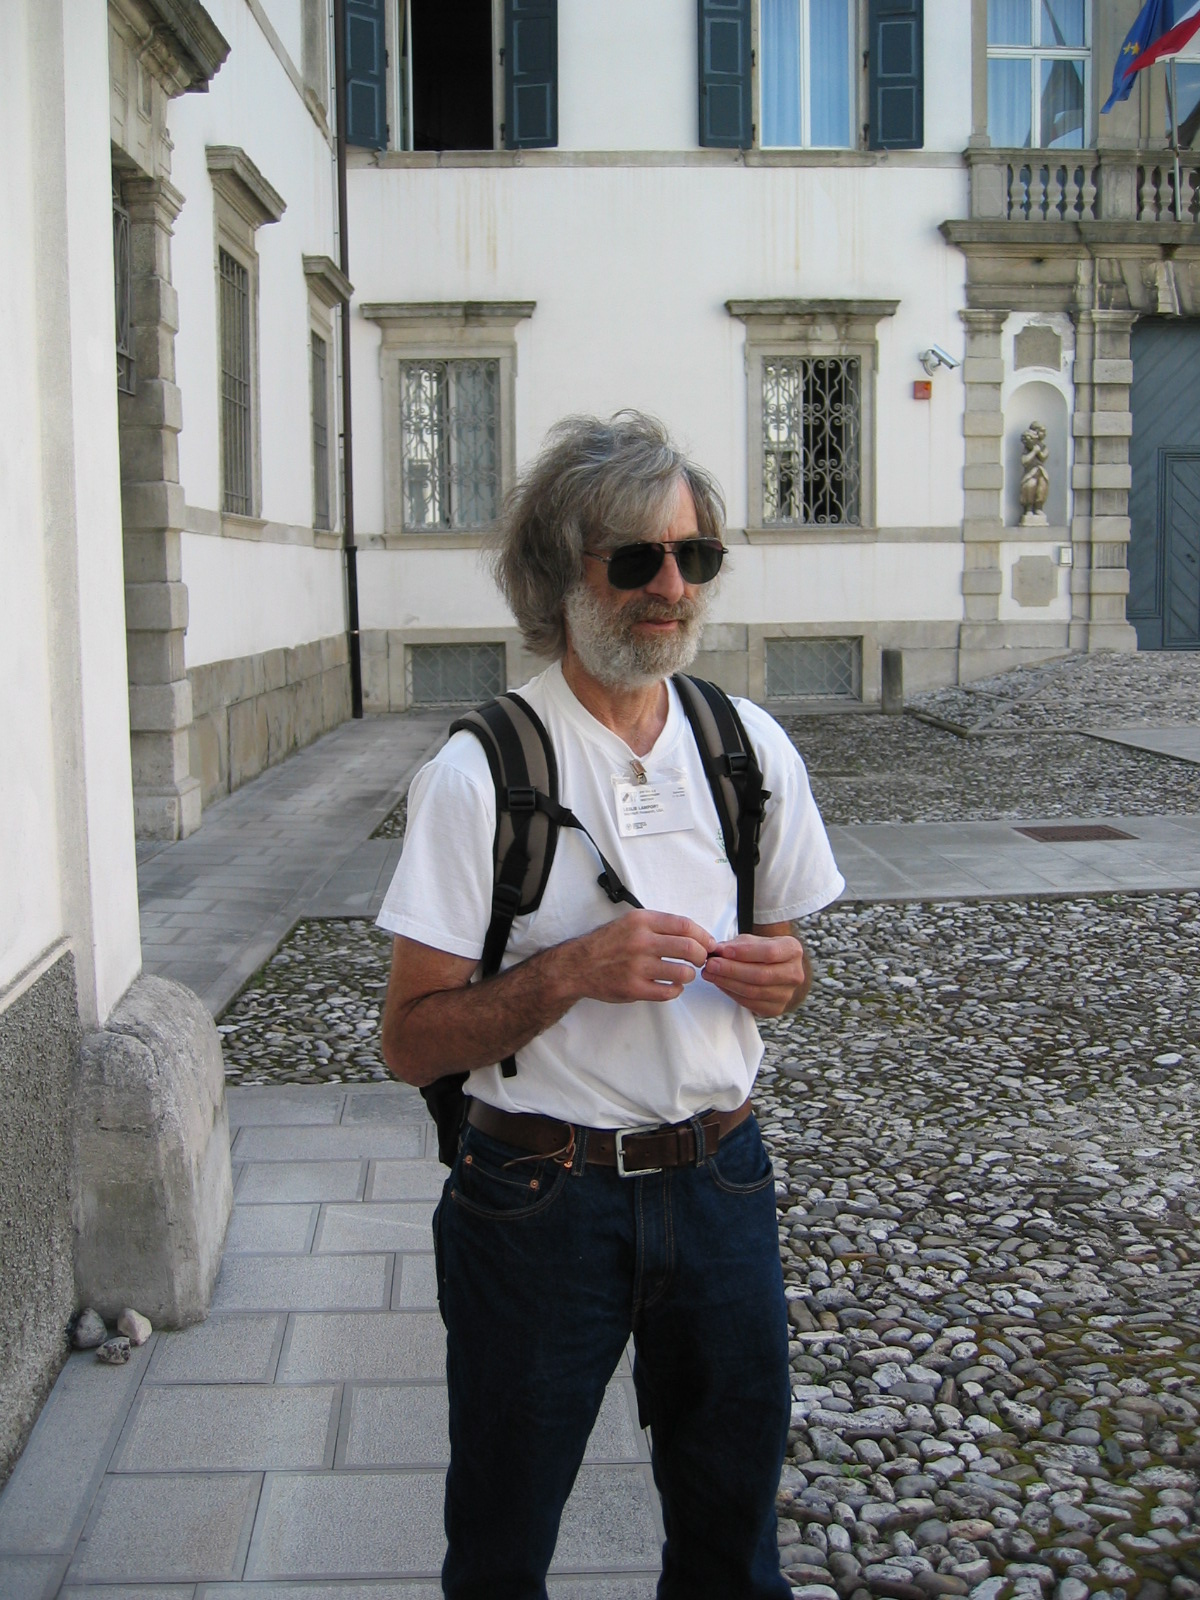
\includegraphics[width=7cm]{figurer/lamport}
  \caption{Leslie Lamport}
  \label{fig:lamport}
\end{figure}

\texttt{tikz} er en pakke, der gør det muligt at beskrive vektorgrafik -- det
er et helt lille programmeringssprog. Figur \ref{fig:tm}
viser et eksempel, der ligger i en særskilt fil (indlæst med
\verb2\input2-kommandoen). 

\begin{figure}[h]
\begin{tikzpicture}[>=latex',join=bevel,]
\tikzstyle{every state}=     [draw=black!50,very thick,fill=gray!20]%
 \node (q0) at (50bp,320bp) [state, initial]{$q_0$};
 \node (q1) at (200bp,320bp) [state]{$q_1$};
 \node (q2) at (350bp,320bp) [state]{$q_2$};
 \node (qacc) at (350bp,240bp) [state]{$q_{\text{\tiny{acc}}}$};
 
\draw[->] (q0) edge[loop above] node[auto]{$a \to \sqcup,R$}(q0);
\draw[->] (q0) edge node[auto]{$b \to R$}(q1);

\draw[->] (q1) edge node[auto]{$\sqcup \to b,L$}(q2);

\draw[->] (q2) edge[loop above] node[auto]{$\begin{array}{c} a \to L \\ b \to L \end{array}$}(q2);

\draw[->] (q2) edge node[auto]{$\sqcup \to R$}(qacc);

\end{tikzpicture}

  \caption{Tilstandsdiagram for Turing-maskine}
  \label{fig:tm}
\end{figure}

%%% Local Variables:
%%% mode: latex
%%% TeX-master: "report"
%%% End:

\chapter{Kildekode} \label{kap:kode}

\texttt{listings}-pakken er særdeles nyttig, hvis man skal have
kildekode med i sin tekst. Listing \ref{listx} viser et første lille
eksempel på hvad man kan.


\begin{lstlisting}[caption={Et eksempel på Java-kode},label=listx,language=Java]
 public class Main {
  public static void main(String[] args) {
    int time = 16;

    if (time < 12) {
      System.out.println("Dingo.");
    } else if (time < 18) {
      System.out.println("Mango.");
    } else {
      System.out.println("Bingo.");
    }
  }
}
\end{lstlisting}

Man kan også definere sine egne environments, så kildekode i bestemte
sprog bliver vist med reserverede ord fremhævet.

%%% Local Variables:
%%% mode: LaTeX
%%% TeX-master: "report"
%%% End:

\chapter{Om krydsreferencer}

Hvis ikke man kender til de rige muligheder for automatisk håndtering
af referencer, som \latex har, er det som at trække rundt på
cykelstien med en dyr racercykel og ærgre sig over, at man ikke kan
komme hurtigere frem, fordi man er nødt til at trække rundt med hvad
man tror er et dårligt designet løbehjul. 

\section{Krydsreferencer} \label{afs:kryds}

Afsnit, underafsnit, tabeller, figurer og formler kan få numre i
\latex. Det gør man med \verb2\label2-kommandoe, som placerer et
mærke. Det kan man senere referere til med en \verb2\ref2. Se efter i
kildeteksten til dette dokument for at lære, hvordan man laver en
henvisning til afsnit \ref{afs:kilder}. 

Det er aldrig nok at skrive \verb2\ref2, for denne kommando skriver
blot nummeret på den label, man henviser til. Jeg har defineret en
kommando \verb2\afs2, der tager et mærke som argument og skriver
"Afsnit'' og nummeret på mærket. Se, hvordan denne kommando er
defineret og brugt. Jeg bruger den også her i \afs{afs:kryds}. 

Pakken \verb2cleveref2 tilbyder en lignende funktionalitet og er værd
at overveje at bruge. 

\section{Kildehenvisninger} \label{afs:kilder}

\begin{ovelse}
  Prøv at skrive
\begin{verbatim}
\bibliographystyle{apalike}
\end{verbatim}
  i stedet for \verb2 \bibliographystyle{plain}2 og se, hvad der
  sker. Hvis du ikke bruger Overleaf, så husk at kompilere to gange. 
\end{ovelse}

%%% Local Variables:
%%% mode: latex
%%% TeX-master: "report"
%%% End:

\chapter{Gode råd}

\section{\latex  kan meget mere end du tror!}

Mange nybegyndere tror, at de skal bruge Word-lignende krumspring for
at få et bestemt udseende. Hvis det ikke lykkes for dem, konkluderer
de ofte, at \latex må lide af alvorlige mangler.

\subsection{Typiske misforståelser}

\begin{itemize}
\item Måske er det layout, man ønsker sig, ikke hensigtsmæssigt. Det
  er almindeligt at man har vaner med sig fra gymnasiet og fra
  Word-land, som snarere skyldes uvaner end stor typografisk
  indsigt. Det er langt bedre at tage ved lære af typografien i
  fagbøger og videnskabelige publikationer end at lade sig styre af en
  gammel SRP-opgave.
  
\item Og der er med meget stor sandsynlighed snarere tale om at der er
  noget, man ikke ved selv, end om noget, det er umuligt at gøre ved
  brug af \latex.
\end{itemize}

\subsection{Noget om layout}

Hvis man \emph{slet ikke} kan acceptere standard-layoutet og drømmer sig
tilbage til SRP-dagene, er der pakken \verb2wordlike2. Her er stor
linjeafstand, Times New Roman, smalle marginer og andet godt, så man
kan genskabe det trygge gymnasielayout og drømme om Word-pølse.

\begin{ovelse}
  Prøv at skrive \verb2\usepackage{wordlike}2 i præamblen, og se hvad
  der sker.
\end{ovelse}

Mange nybegyndere tror også, at de er nødt til at lave manuelle
krumspring mange steder i et dokument for at styre dets layout. Typisk
ved de ikke, at \verb2report2-dokumentklassen findes og kender kun
\verb2article2. Derfor bruger de tvungne sideskift med
\verb2\newpage2. Nybegyndere synes også ofte, at der skal være større
afstand mellem paragraffer og indsætter tvungne linjeskift med
\verb2\\2 overalt.

Dette er en anden typisk arv fra Word-land, hvor man er nødt til at
skulle håndtere den slags manuelt rundt om i Word-pølsen. Men i \latex
er der en masse parametre, der bestemmer marginbredde, linjeafstand
mm. Dem kan man selv sætte én gang for alle oppe i præamblen, så man
ved en lille ændring dér kan ændre dokumentets layout fuldstændig.

Se også
\url{https://da.overleaf.com/learn/latex/Articles/How_to_change_paragraph_spacing_in_LaTeX},
der forklarer de forskellige parametre, og hvordan man sætter dem ét
sted i dokumentet.

Her er nogle små øvelser, der viser hvad parametrene kan.

\begin{ovelse}
  Prøv at skrive \verb2\documentclass[a4paper,11pt,twocolumn]{report}2 i præamblen og se,
  hvad der sker.
\end{ovelse}

\begin{ovelse}
  Prøv at skrive
\begin{verbatim}
\setlength{\parskip}{4mm}
\end{verbatim}
  i præamblen og se, hvad der sker.
\end{ovelse}

\begin{ovelse}
  Prøv at skrive
\begin{verbatim}
\setlength{\parindent}{0mm}
\end{verbatim}
  i præamblen og se, hvad der sker.
\end{ovelse}

\begin{ovelse}
  Prøv at skrive
  \begin{verbatim}
\renewcommand\baselinestretch{1.5}
\end{verbatim}
  i præamblen og se, hvad der sker.
\end{ovelse}

%%% Local Variables:
%%% mode: latex
%%% TeX-master: "report"
%%% End:


\bibliography{litteratur}
\bibliographystyle{apalike}

\appendix

\chapter{Her er præamblen}

\begin{lstlisting}
% HER BEGYNDER PRÆAMBLEN

% Skrivemaskinfont

\usepackage{courier}

% Farver

\usepackage{color}

\usepackage{listings}

\newcommand{\injava}[1]{\lstinline[language=Java]{#1}}

\lstnewenvironment{java} {\lstset{language=Java}} {}

% En pakke til lokalisering, herunder orddeling på andre sprog end
% amerikansk engelsk

\usepackage[danish]{babel}

% En nyttig matematik-pakke

\usepackage{amsmath}

% En anden nyttig pakke -- til opsætning af matematiske sætninger,
% definitioner mm.

\usepackage{amsthm}

% Symboler

\usepackage{amssymb}

% Ved brug af billedfiler

\usepackage{graphicx}

% Til hyperlinks

\usepackage{hyperref}

% Til ombrydning af lange URL'er

\usepackage{breakurl}
\usepackage{xspace}

% Til TikZ

\usepackage{tikz}

% Til automater i TikZ

\usetikzlibrary{arrows,shapes, calc}
\usetikzlibrary{automata}

% FILEN MED KOMMANDOER

%%% Local Variables:
%%% mode: LaTeX
%%% TeX-master: "report"
%%% End:

% Baseret på https://gist.github.com/mpdehnel/cc43e89a09c18ef6a602

\definecolor{mygreen}{rgb}{0,0.6,0}
\definecolor{mygray}{rgb}{0.5,0.5,0.5}
\definecolor{mymauve}{rgb}{0.58,0,0.82}
\definecolor{verylightgray}{gray}{0.92}

\lstset{ %
  backgroundcolor=\color{verylightgray},     % Baggrundsfarve; kræver pakken
                                                               % color - dvs. \usepackage{color} eller \usepackage{xcolor}
  basicstyle=\footnotesize\ttfamily,   % Skrivemaskine-font
  breakatwhitespace=false,                 % Intet linjeskift ved whitespace
  breaklines=true,                                % Automatisk linjeskift
  captionpos=b,                                    % Caption sat nederst i bunden
  commentstyle=\color{mygreen},     % Kommentarer med grøn
  escapeinside={\%*}{*)},                     % LaTeX-escape til hvis
                                                               % man får brug for LaTeX-kommandoer i koden
  extendedchars=true,                         % Tillader ikke-ASCII-tegn. Virker IKKE med UTF-8.
  frame=single,                                      % Ramme om koden.
  keywordstyle=\color{blue},               % Reserverede ord med blåt
  numbers=left,                                     % Linjenummerering mod venstre
  numbersep=5pt,                                % Afstand mellem linjenumre og kode
  numberstyle=\tiny\color{mygray},   % LInjenumre med grå
  rulecolor=\color{black},                     
  showspaces=false,                             
  showstringspaces=false,           
  showtabs=false,
  stepnumber=1,                    % Hver linje får et nummer
  stringstyle=\color{mymauve},     
  tabsize=2,
  title=\lstname                   
}

%%% Local Variables:
%%% mode: latex
%%% TeX-master: "report"
%%% End:

\newcommand{\bibtex}{\mbox{\textsc{BiB}\TeX}\xspace}
\newcommand{\latex}{\LaTeX\xspace}

\newcommand{\fig}[1]{Figur \ref{#1}}
\newcommand{\afs}[1]{Afsnit \ref{#1}}

\newcommand{\svar}{\paragraph{Svar:}}

\theoremstyle{definition}
\newtheorem{ovelse}{Øvelse}[chapter]

%%% Local Variables:
%%% mode: latex
%%% TeX-master: "report"
%%% End:


\end{lstlisting}
%%% Local Variables:
%%% mode: LaTeX
%%% TeX-master: "report"
%%% End:


\end{document}

%%% Local Variables:
%%% mode: latex
%%% TeX-master: t
%%% End:
